\section{Computational Results}\label{sec:compResults}
In this section we show several computational experiments using the Euler
equations to demonstrate the properties of SRD. We will also use these
examples to examine 
properties of different gradient choices and base schemes. 
%We solve the conservation law \eqref{eq:conslaw2D} with different fluxes $\mathbf{F}$, to include both smooth and discontinuous
%solutions.

%\subsection{Linear fluxes}
%\subsubsection{Linear convergence study}
%We solve \eqref{eq:conslaw2D} with the flux $\mathbf{F}(u) = [-2\pi y u, 2\pi x u]$ and initial condition
%$$
%u_0(x,y) = w(\theta - \pi/2)
%$$
%where
%$$
%w(\theta) = \frac{1}{2}\left( \text{erf}\left( \frac{\pi/6 - \theta}{\sqrt{4/100}} \right) + \text{erf}\left( \frac{\pi/6 + \theta}{\sqrt{4/100}} \right)\right)
%$$
%until the final time $T = 1$ on the domain enclosed by two concentric disks of 
%radii $R_1 = 0.751$ and $R_2 = 1.251$.  
%Figure \ref{fig:rotatinghillgrid} shows the computational domain 
%embedded in a $50 \times 50$ grid.  The exact solution is the initial condition 
%rotated about the point $(1.5,1.5)$, where $T=1$ corresponds to one solid 
%body rotation. This example IS FROM \cite{}, for comparison.  (AND ADD
%COMPARISON - ARE THEY OR WE MORE ACCURATE< BUT WE ARE EASIER).   
%The errors 
%measured in the $L_1$ and $L_\infty$ norms are provided in 
%Tables \ref{tab:ex1_L1} and \ref{tab:ex1_Linf}.  Figure
%\ref{fig:rotatinghillexactiso} shows isolines of solution at the initial 
%and final time.  The exact solution is applied as the boundary condition.
%CHEATING?
%This problem is solved using the finite volume TVD-RK2 scheme. 
%
%\begin{figure}
%\subfloat[$50\times50$ grid and annulus domain.]{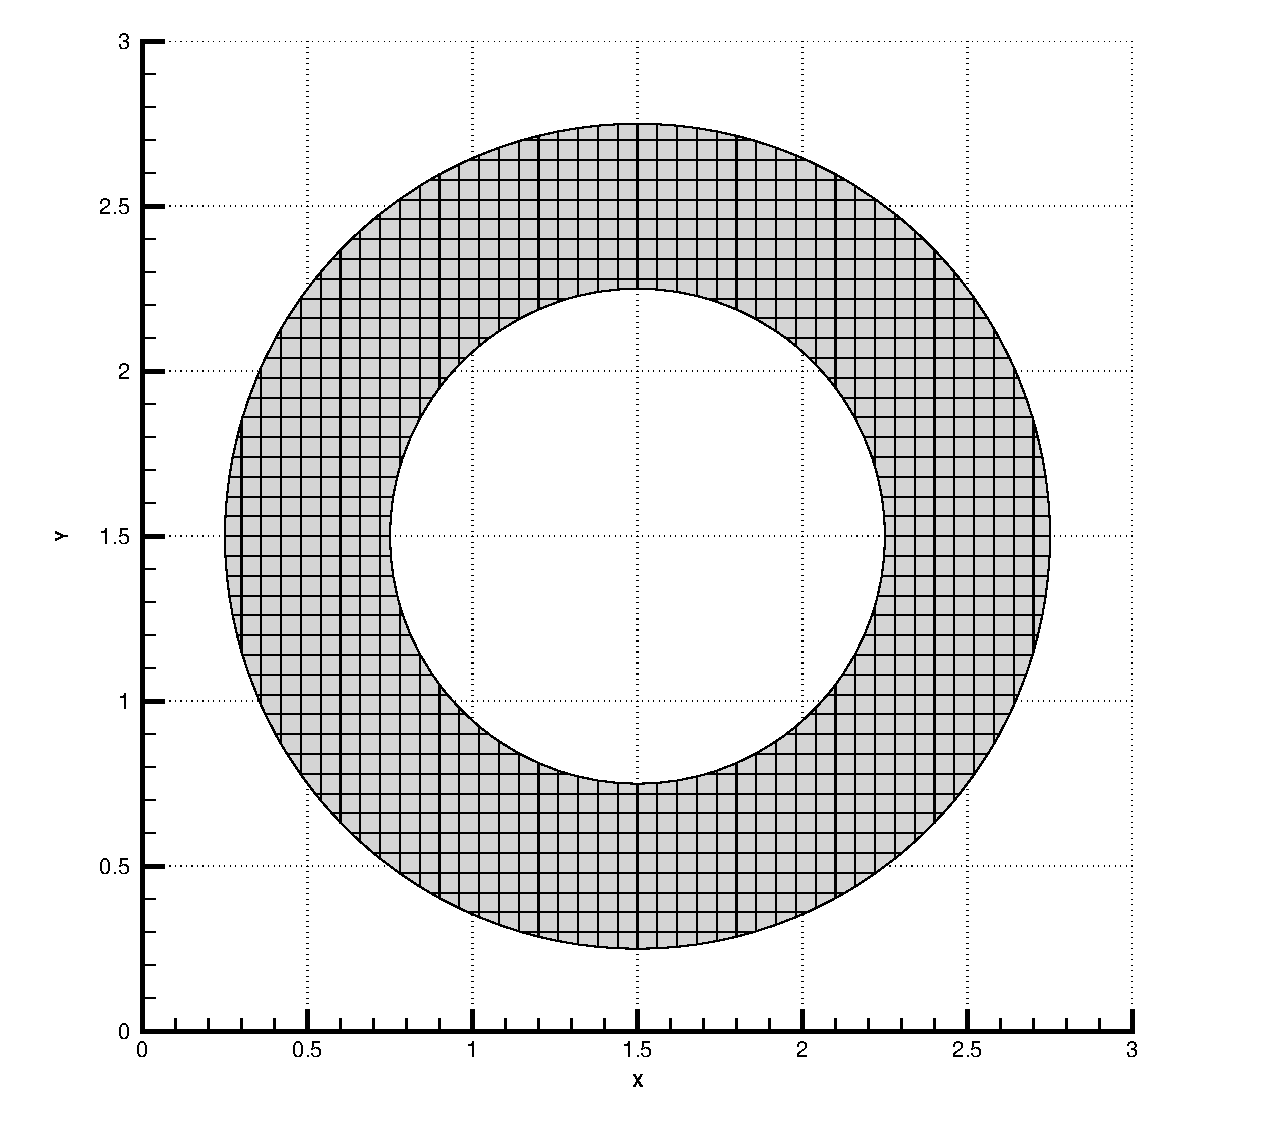
\includegraphics[width = 0.5\linewidth]{figs/rotatinghill_grid.eps} \label{fig:rotatinghillgrid}} 
%\quad
%\subfloat[Isolines of exact solution at the initial and final time. SHOW
%COMPUTED SOLUTION TOO]{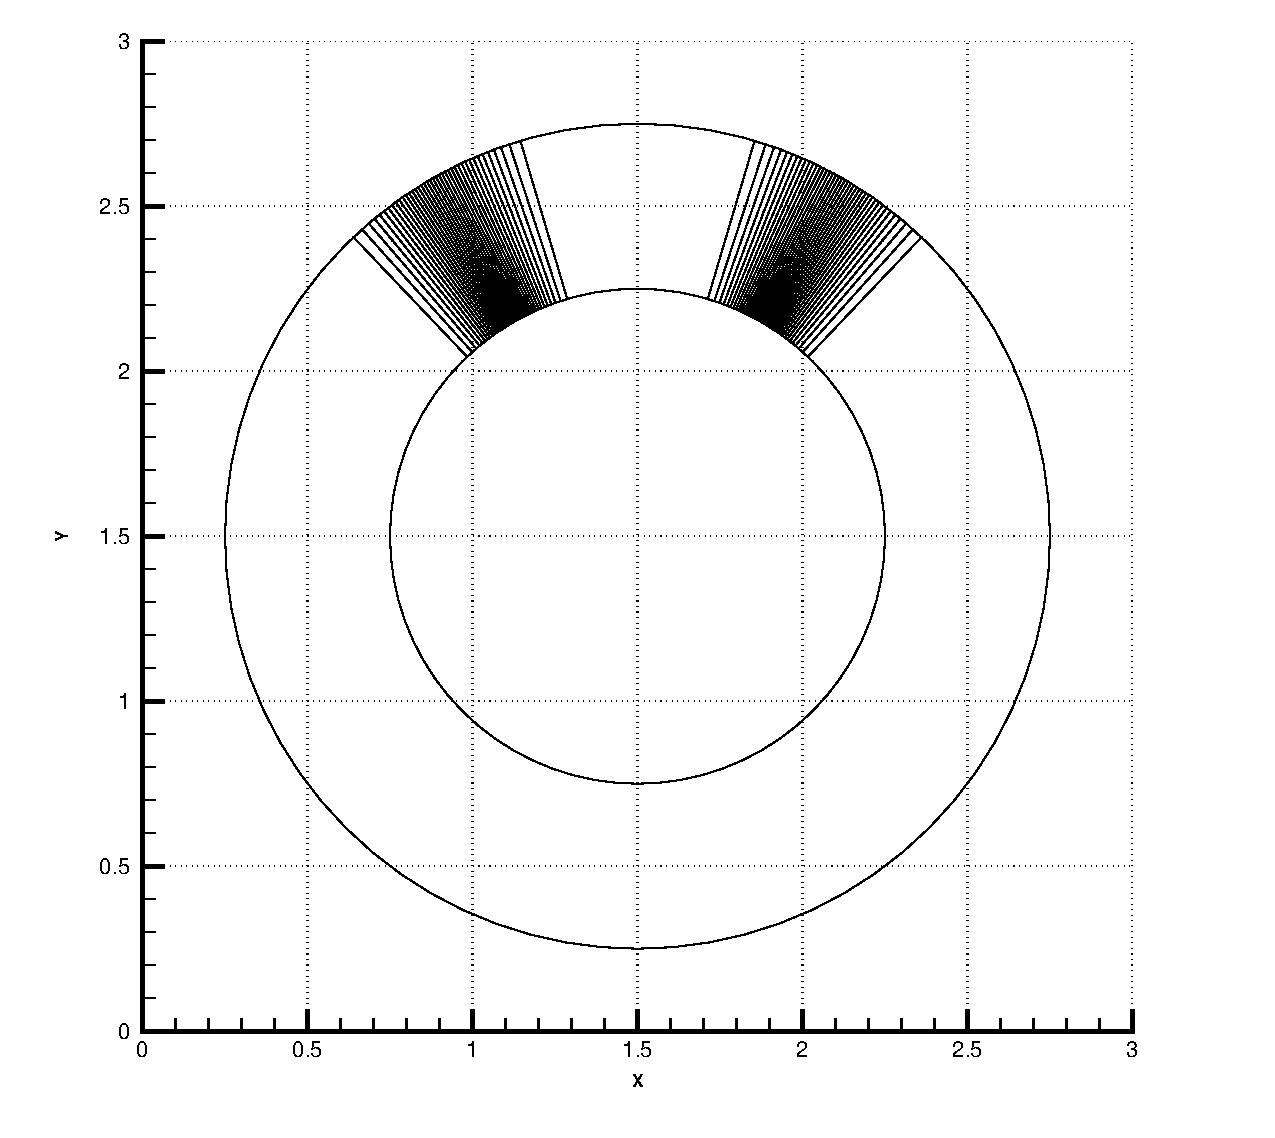
\includegraphics[width = 0.5\linewidth]{figs/rotatinghill_solution.eps}\label{fig:rotatinghillexactiso}}
%\end{figure}
%    % \caption{}\label{tab:ex1_L1}
%
%{\large
%\begin{table}
%\centering
%\subfloat[$L_1$ errors. \label{tab:ex1_L1}]{
%    \begin{tabular}{|c|c|c|c|c|}
%        \hline
%         $N_x \times N_y$ & $p = 0$ & $p=1$& $p=2$ & $p=3$ \\
%         \hline
%         50 & 2.3937e-1(-) &  5.6588e-2  (-)& 4.1690e-2  (-)&   2.0694e-2 (-)\\
%         \hline
%         100 &  1.5521e-1 (0.62) &  2.0125e-2  (1.49)& 7.8165e-3 (2.41)& 1.6813e-3 (3.62)\\
%         \hline
%         200 &  9.4138e-2 (0.72) & 5.5222e-3 (1.86)&  9.98411e-4 (2.96)& 8.8527e-5 (4.24)\\
%        %  \hline
%        %  400 &  () &  ()&  ()&  ()\\
%         \hline
%    \end{tabular}
%    }
%\quad
%\subfloat[$L_\infty$ errors. \label{tab:ex1_Linf}]{
%    \begin{tabular}{|c|c|c|c|c|}
%        \hline
%         $N_x \times N_y$ & $p = 0$ & $p=1$& $p=2$ & $p=3$ \\
%         \hline
%         50 & 3.0385e-1 (-) &  1.6856e-1 (-)& 1.1809e-1 (-)&  7.0682e-2 (-)\\
%         \hline
%         100 & 2.3332e-1 (0.38) & 8.5487e-2 (1.04)& 5.1249e-2 (1.20)& 1.6657e-2 (2.08)\\
%         \hline
%         200 &  1.7698e-1 (0.39) & 3.4940e-2 (1.29)& 1.4500e-2 (1.82)&  1.9507e-3 (3.09)\\
%        %  \hline
%        %  400 &   () &  ()&  ()&  ()\\
%         \hline
%    \end{tabular}
%    }
%
%\caption{Errors for the linear convergence study. ADD METHOD DETAILS TO
%DESCRIPTION - USED WHICH GRADIENT RECON. ADD 400 POINTS}
%\end{table}
%}
%
%\subsubsection{Overlapping neighborhoods}
%The purpose of this example is to demonstrate that our algorithm can handle a substantial number of overlapping neighborhoods.  
%Using the streamfunction
%$$
%\phi = R - 0.25\sin(10\theta),
%$$
%with $R = \sqrt{(x-1.5)^2+(y-1.5)^2}$ and $\theta = \arctan((y-1.5)/(x-1.5))$, we define a linear flux based on the resulting divergence free velocity field, i.e.,  $\mathbf{F}(u) = [\phi_y u, -\phi_xu]$.  The characteristics of \eqref{eq:conslaw} lie on the isolines of the streamfunction.
%
%A steady state solution to \eqref{eq:conslaw} with the above flux is given by the streamline function.  Therefore, we start with the initial condition given by the streamline function $\phi$, and compute the solution until the final time $T = 10$ on a $100 \times 100$ grid.  Additionally, we set the flux normal the domain boundary $\mathbf{F}\cdot \mathbf{n} = 0$.  This is to ensure that information does not leave the domain and should solution growth occur, this will more easily be noticed.
%This problem is solved using the finite volume TVD-RK2 scheme. 
%
%
%\begin{table}[h]
%    \centering
%    \subfloat[$L_1$ errors.]{
%    \begin{tabular}{|c|c|c|c|}
%    \hline
%        $p = 0$ & $p =1$ & $p = 2$ & $p =3$  \\
%        \hline
%        3.8585e-1 & 3.6118e-2 & 8.29907e-3 & 4.3116e-3\\
%        \hline
%    \end{tabular} \label{tab:errorsteadystatel1}
%    }
%    \quad
%\subfloat[$L_\infty$ errors.]{
%    \begin{tabular}{|c|c|c|c|}
%    \hline
%        $p = 0$ & $p =1$ & $p = 2$ & $p =3$  \\
%        \hline
%        2.9470e-1 & 9.5323e-2 & 2.4851e-2 &  5.4720e-3 \\
%        \hline
%    \end{tabular}
%    \label{tab:errorsteadystatelinfty}
%    }
%    
%\caption{Errors for overlapping neighborhoods study.} \label{tab:overlappingerrors}
%\end{table}
%
%\begin{figure}[h]
%%\subfloat[Isolines of exact solution at the initial and final time.]{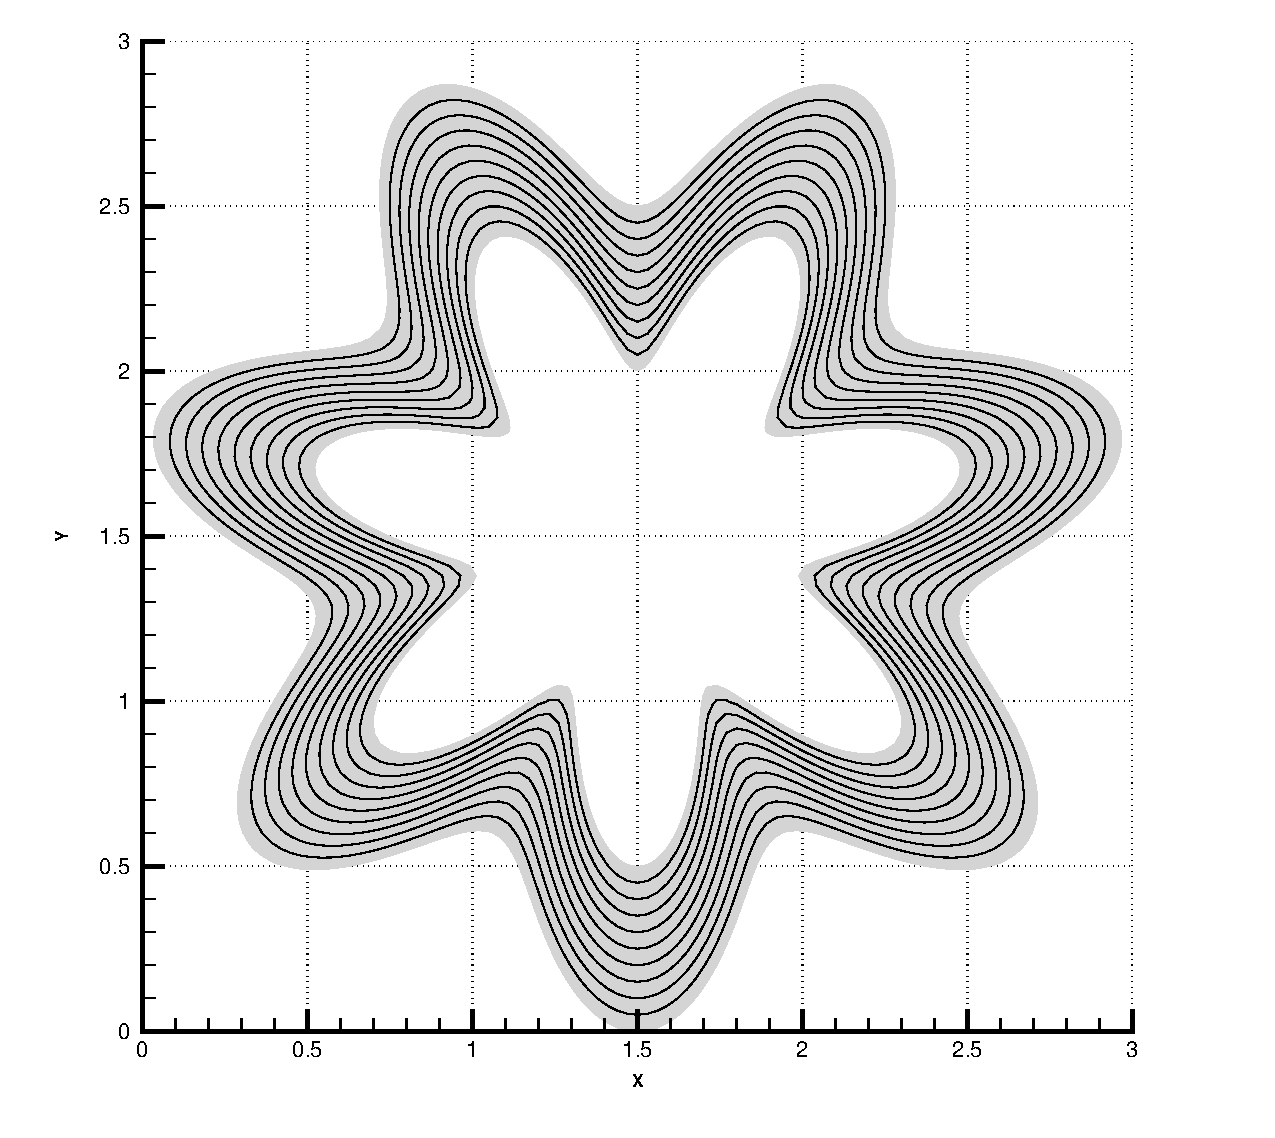
\includegraphics[width = 0.5\linewidth]{figs/waveyiso.eps} \label{fig:waveyisolines}} 
%%\subfloat[Isolines of exact solution at the initial and final time.]{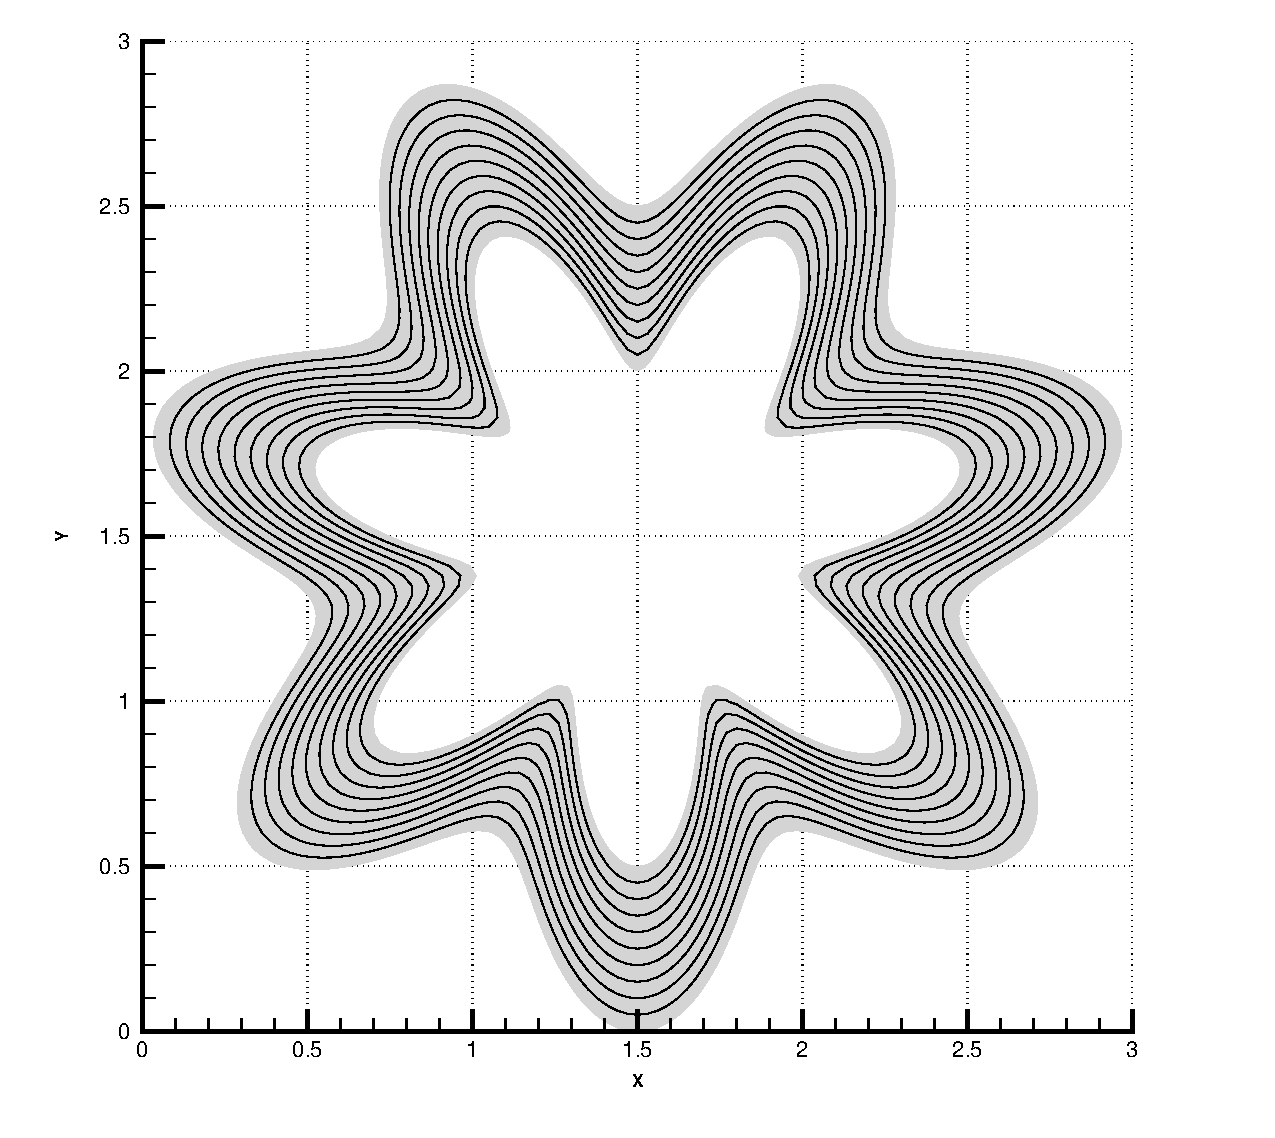
\includegraphics[width = 0.5\linewidth]{figs/waveyiso.eps} \label{fig:waveyisolines}} 
%%\quad
%\subfloat[Number of overlapping merging neighborhoods: one (blue), two (green), three (red).]{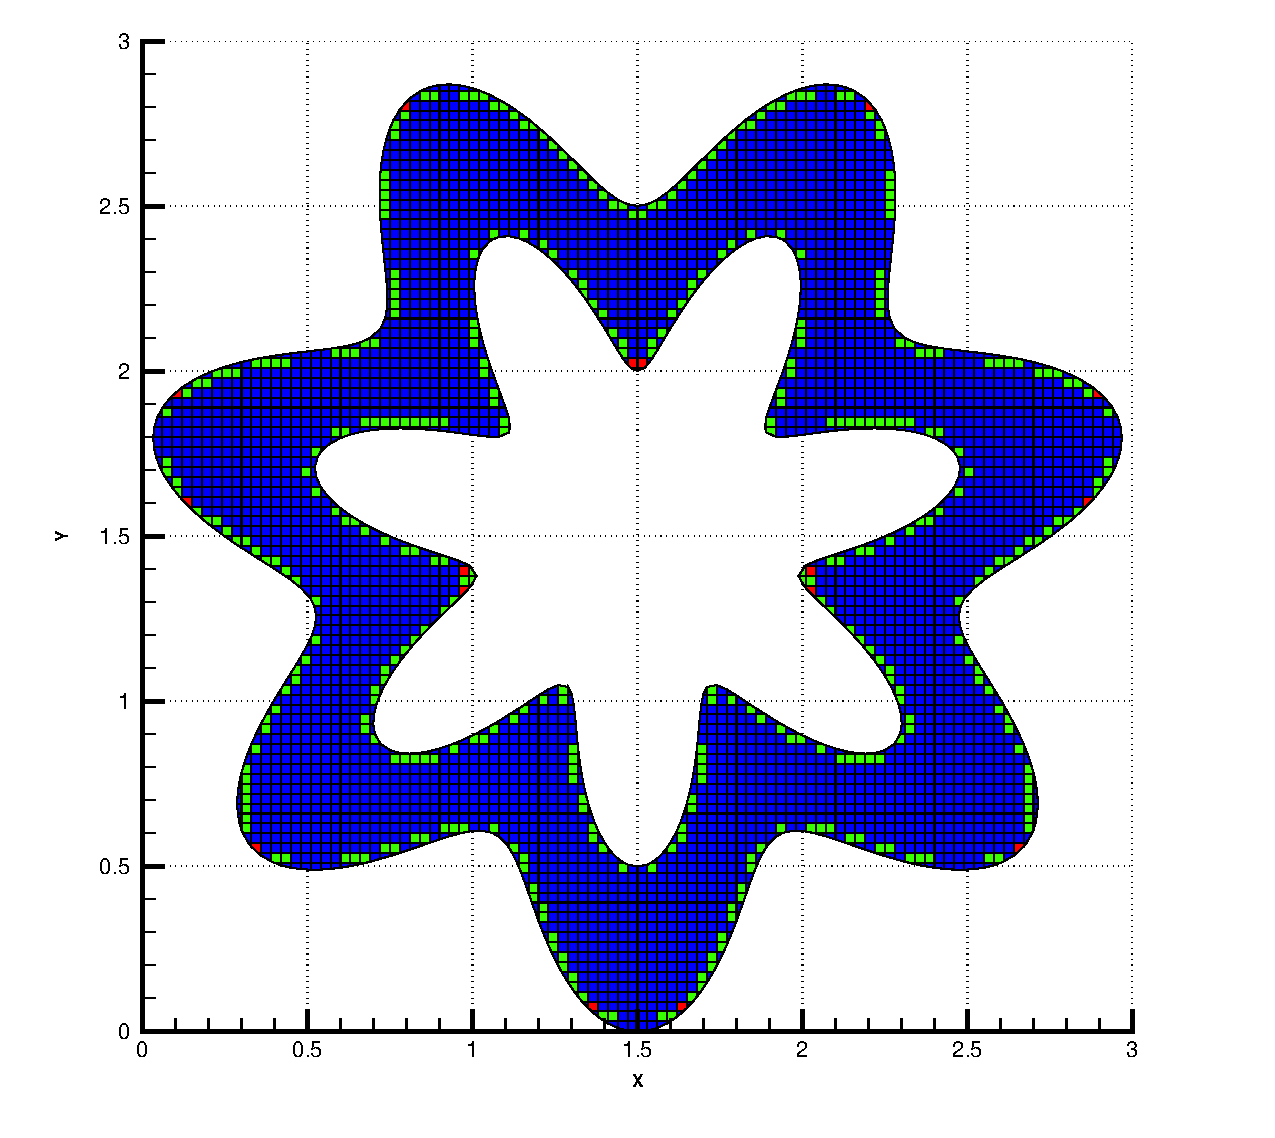
\includegraphics[width = 0.5\linewidth]{figs/waveynumhoods.eps}\label{fig:waveynumhoods}}
%% 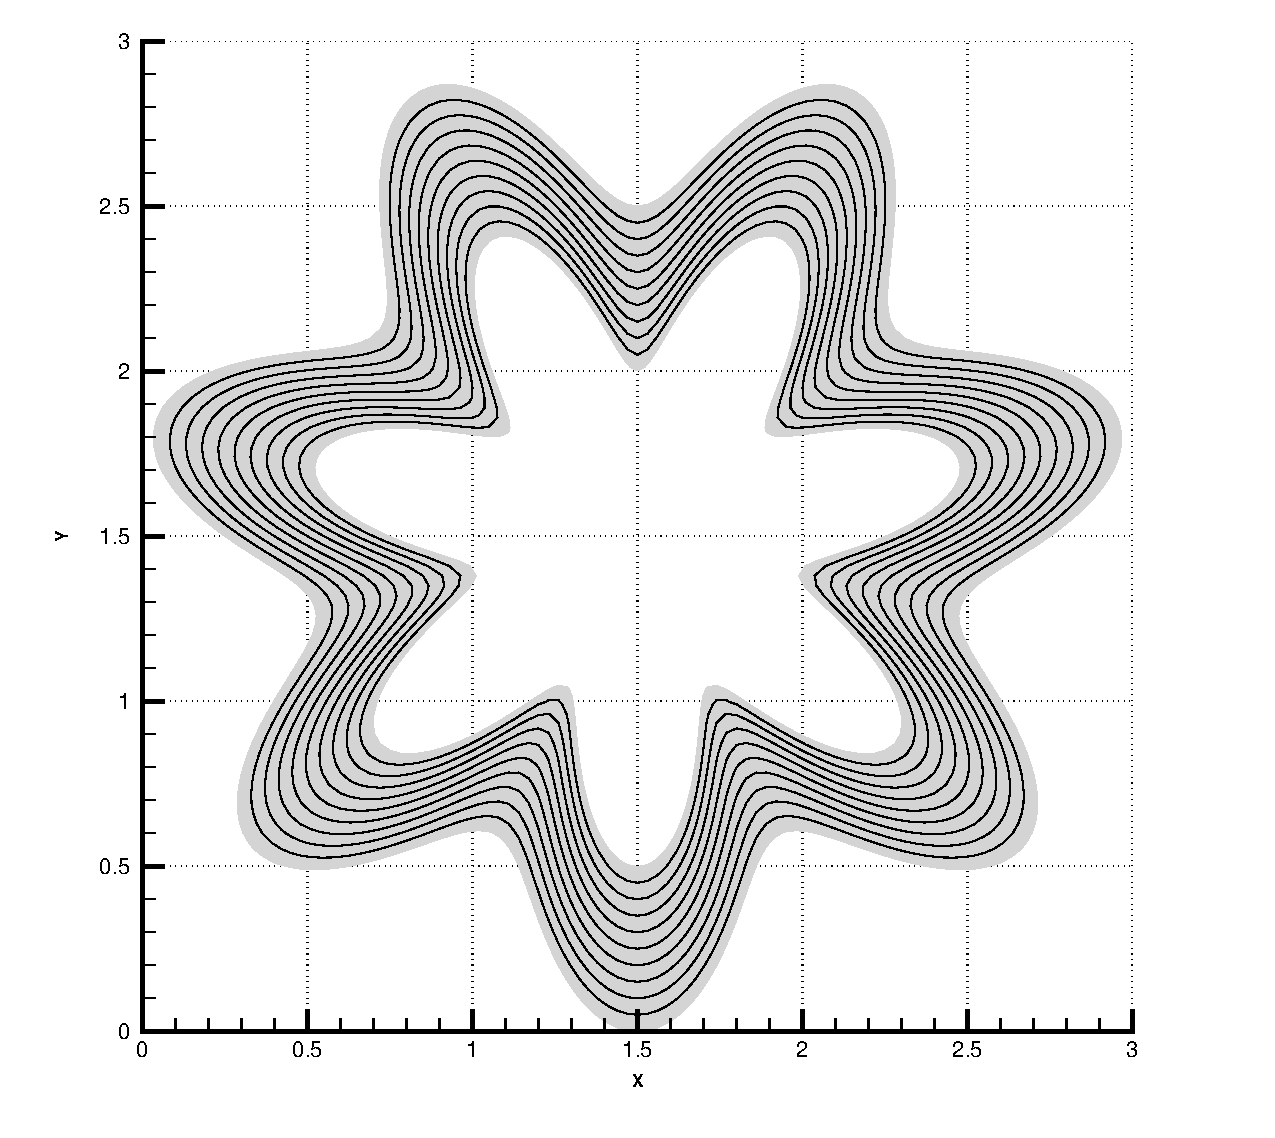
\includegraphics[width = 0.5\linewidth]{figs/waveyiso.eps} 
%\subfloat[Isolines of exact solution at the initial and final time.]{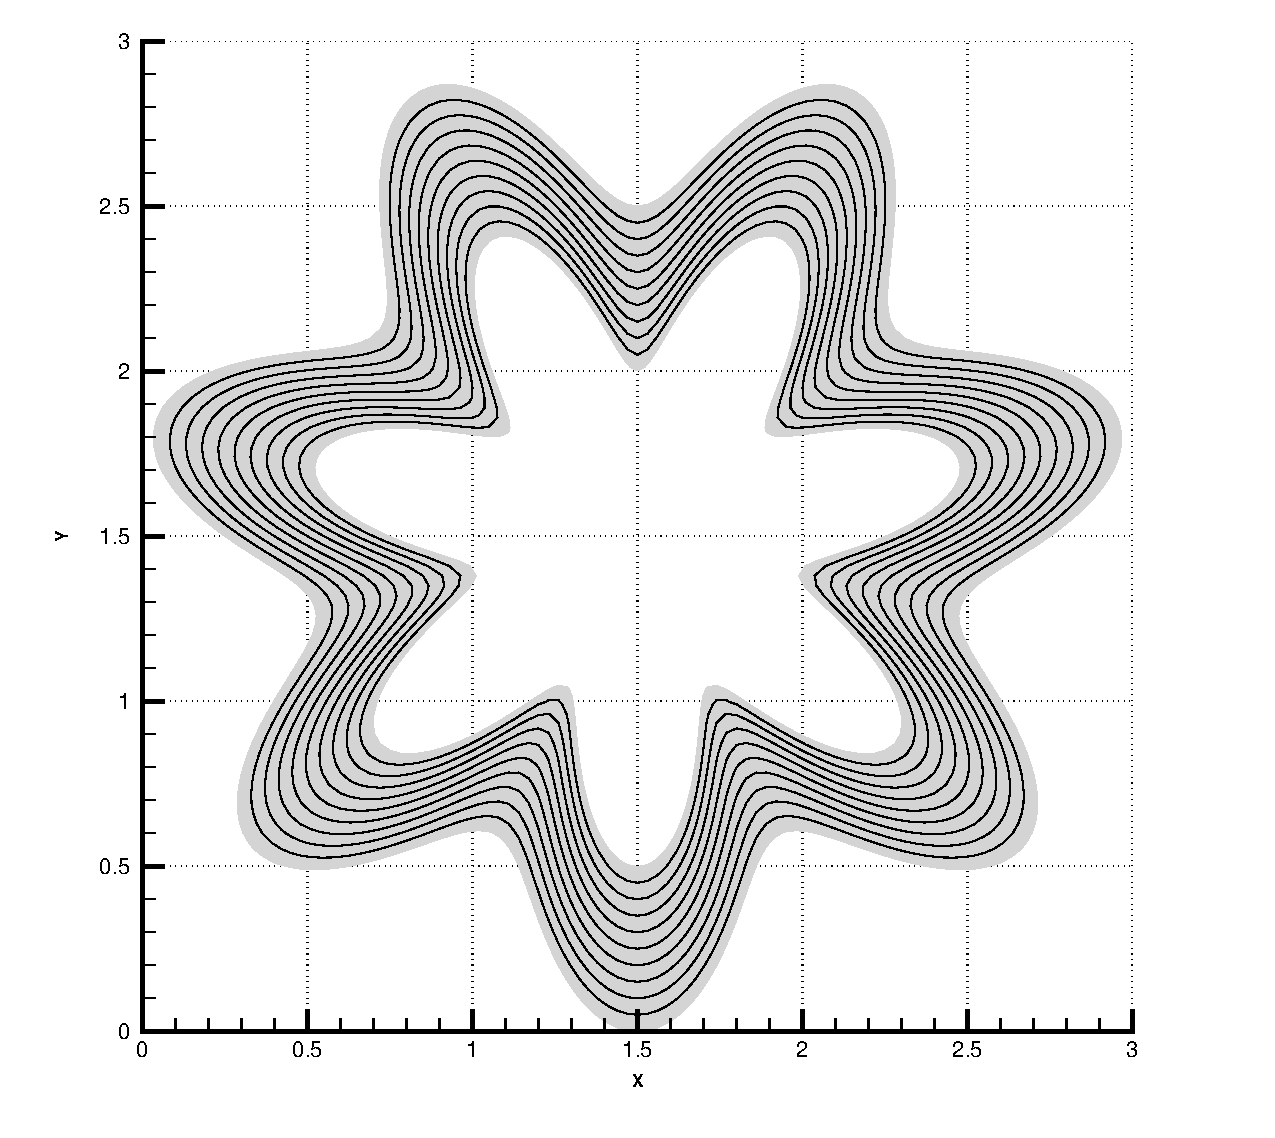
\includegraphics[width = 0.5\linewidth]{figs/waveyiso.eps} \label{fig:waveyisolines}} 
%\caption{Isolines of exact solution at the initial and final time for the
%wavy domain with overlapping neighborhoods. CANT SEE COLORS. WHAT DOES
%THIS EX ADD FROM PREVIOUS ONE} 
%% \label{fig:overlappingneighborhoods}
%% \label{fig:waveyisolines}} 
%\end{figure}
%
%In Figure \ref{fig:waveyisolines}, we show the isolines of the exact solution at the initial and final times.  Additionally, Figure \ref{fig:waveynumhoods} shows the number of overlapping neighborhoods on each cell.  In this example, we have at most three overlapping neighborhoods.  They are concentrated where the boundary has high curvature.   We do not observe growth in the numerical solution as indicated by $L_1$, $L_\infty$ errors of the solution at the final time listed in Table \ref{tab:overlappingerrors}.  Although this experiment does not prove stability of our numerical scheme, not observing unbounded growth in the numerical solution is a necessary condition.


%\subsection{Nonlinear fluxes}
\subsection{Supersonic vortex study}
We compute the solution to a supersonic flow 
through a quarter circle.  This problem has often been used in accuracy 
studies \cite{aftosmis:acc} since it has an exact solution given by 
$$
\begin{pmatrix}
\rho\\
u \\
v \\
p
\end{pmatrix} = 
\begin{pmatrix}
\left ( 1 + 1.0125(1-r^{-2}) \right)^{2.5}\\
2.25r^{-1}\sin(\theta)\\
-2.25r^{-1}\cos(\theta)\\
\frac{1}{\gamma}\rho^{\gamma}
\end{pmatrix},
$$
where $r = \sqrt{x^2+y^2}$. The inner radius is $r = 1.0$ and the outer radius
is $r = 1.384$. The second order MOL scheme is used, and we march
to steady state, until the maximum density update is below $10^{-10}$.  
The exact solution is used to set the ghost cells at the inflow and
outflow boundaries. The domain size is 1.43 by 1.4301 (slightly different
to prevent mesh  degeneracies).  

We also use this example to compare the accuracy of two different formulations
for the cut cell gradients, and the effect of state redistribution versus 
marching to steady state using local time-stepping without SRD.  
For first order gradients, we use a linear least squares reconstruction for
both the irregular cell gradient (cut cells and their one-away neighbors) described in , and the SRD gradients, which update the cut cell solution after stabilization. Second order accurate gradients fit a quadratic for both
the cut cells and tiles, but only the first derivative terms are used for 
the gradients. The second order derivatives are subsequently ignored.  More information about the first and second order gradient reconstructions can be found in Sections \ref{sec:limit} and \ref{sec:srd_postprocessing}.

The $L_1$ norm of the error in the volume is $\sum_{i,j} \,
V_{ij} \lvert e_{ij } \rvert$ and at the boundary is $ \sum_{{i,j} \in \partial \Omega} \, A_{ij} \lvert e_{ij
} \rvert$ where $A_{ij}$ is the length of the boundary segment in cut cell $(i,j)$.
These are given in Table \ref{tab:ex1_L1vol} and \ref{tab:ex1_L1bndry}. 


\begin{table}[h]
	\hspace*{-.5in}
	\subfloat[$L_1$ volume errors. \label{tab:ex1_L1vol}]{
		\begin{tabular}{|c|l|l||l|l|}
			\hline
			$N_x ,N_y$ & \multicolumn{2}{|c||}{Local Time Stepping (no SRD)} & \multicolumn{2}{|c|}{State Redistribution}  \\
			\hline
			& 1st order gradients & 2nd order gradients & 1st order gradients & 2nd order gradients \\
			\hline
			27 & 6.09e-3  & 2.58e-3 & 6.75e-3 & 2.76e-3 \\
			\hline
			54  & 1.67e-3  (3.6)  & 6.39e-4 (4.0) & 1.78e-4 (3.8)  & 6.38e-4 (4.3) \\
			\hline
			108 & 3.41e-3  (4.9)  & 1.50e-4 (4.3) & 3.63e-4 (4.9)  & 1.53e-4 (4.2) \\
			\hline
			216 & 6.62e-5  (5.2)  & 3.61e-5 (4.2) & 6.52e-5 (5.6)  & 3.65 e-5  (4.2)\\
			\hline
			432 & 1.34e-5  (4.9)  & 8.70e-6 (4.1) & 1.40e-5 (4.7)  & 8.85 e-6  (4.1)\\
			\hline
			864 & 2.59e-6  (5.2)  & 2.11e-6 (4.1) & 2.68e-6 (5.2)  & 2.15 e-6  (4.1)\\
			\hline \hline
		\end{tabular}
	}
	\quad
	\vspace*{.2in}
	
	\hspace*{-.5in}
	\subfloat[$L_1$ boundary errors. \label{tab:ex1_L1bndry}]{
		\begin{tabular}{|c|l|l||l|l|}
			\hline
			$N_x , N_y$ & \multicolumn{2}{c||}{Local Time Stepping (no SRD)} & \multicolumn{2}{c|}{State Redistribution}  \\
			\hline
			& 1st order gradients & 2nd order gradients & 1st order gradients & 2nd order gradients \\
			\hline
			27  &  6.75e-02       &   3.41e-02 &  6.84e-02 &  3.31e-02 \\
			\hline
			54  &  2.79e-02  (2.4) &   1.27e-02 (2.7)  &  2.83e-02 (2.4) &  1.21e-02 (2.7) \\
			\hline
			108 &  1.00e-02  (2.8) &   4.81e-03  (2.7) &  1.03e-02  (2.8)&  4.69e-03 (2.6)\\
			\hline
			216 &  3.51e-03  (2.9) &   1.88e-03  (2.6) &  3.65e-03  (2.8)&  1.82e-03 (2.6) \\
			\hline
			432 &  1.21e-03  (2.9) &   7.23e-04 (2.6)  &  1.24e-03  (3.0)  &  7.18e-04 (2.6) \\
			\hline
			864 &  3.78e-04  (3.2) &   2.82e-04 (2.6)  &  3.96e-04  (3.1)  &  2.85e-04 (2.6) \\
			\hline \hline
		\end{tabular}
	}
	
	\caption{\sf L1 norm of the error in the domain volume and along the boundary, for the supersonic
		vortex example.}
\end{table}

Note that the error at the cut cells is larger than in the volume cells, and has a
slower convergence rate. Since they are of lower dimension, the $L_1$
accuracy in the entire flow field is still second order.  At the boundary,
Richardson extrapolation shows that the convergence rate is seems to be
between 1.38 and 1.5.
This has also been found in other cut cell studies \cite{XX}, and is not due to
SRD.

Figure \ref{fig:ssv} shows that using second order cut cell gradients is about
a factor of 2 more accurate on coarser grids. Ultimately the gradient
error is reduced, and the  curves approach each other. 
Figure \ref{fig:ssv} also shows a comparison of the error in the converged
solution using local time stepping without SRD, and the error with full timesteps and
SRD stabilization, for both first and second order gradients.
The curves lie on top of each other, showing that 
SRD does not degrade the computed solution with too much diffusion due
to the merging neighborhoods.

\begin{figure}
	\begin{center}
		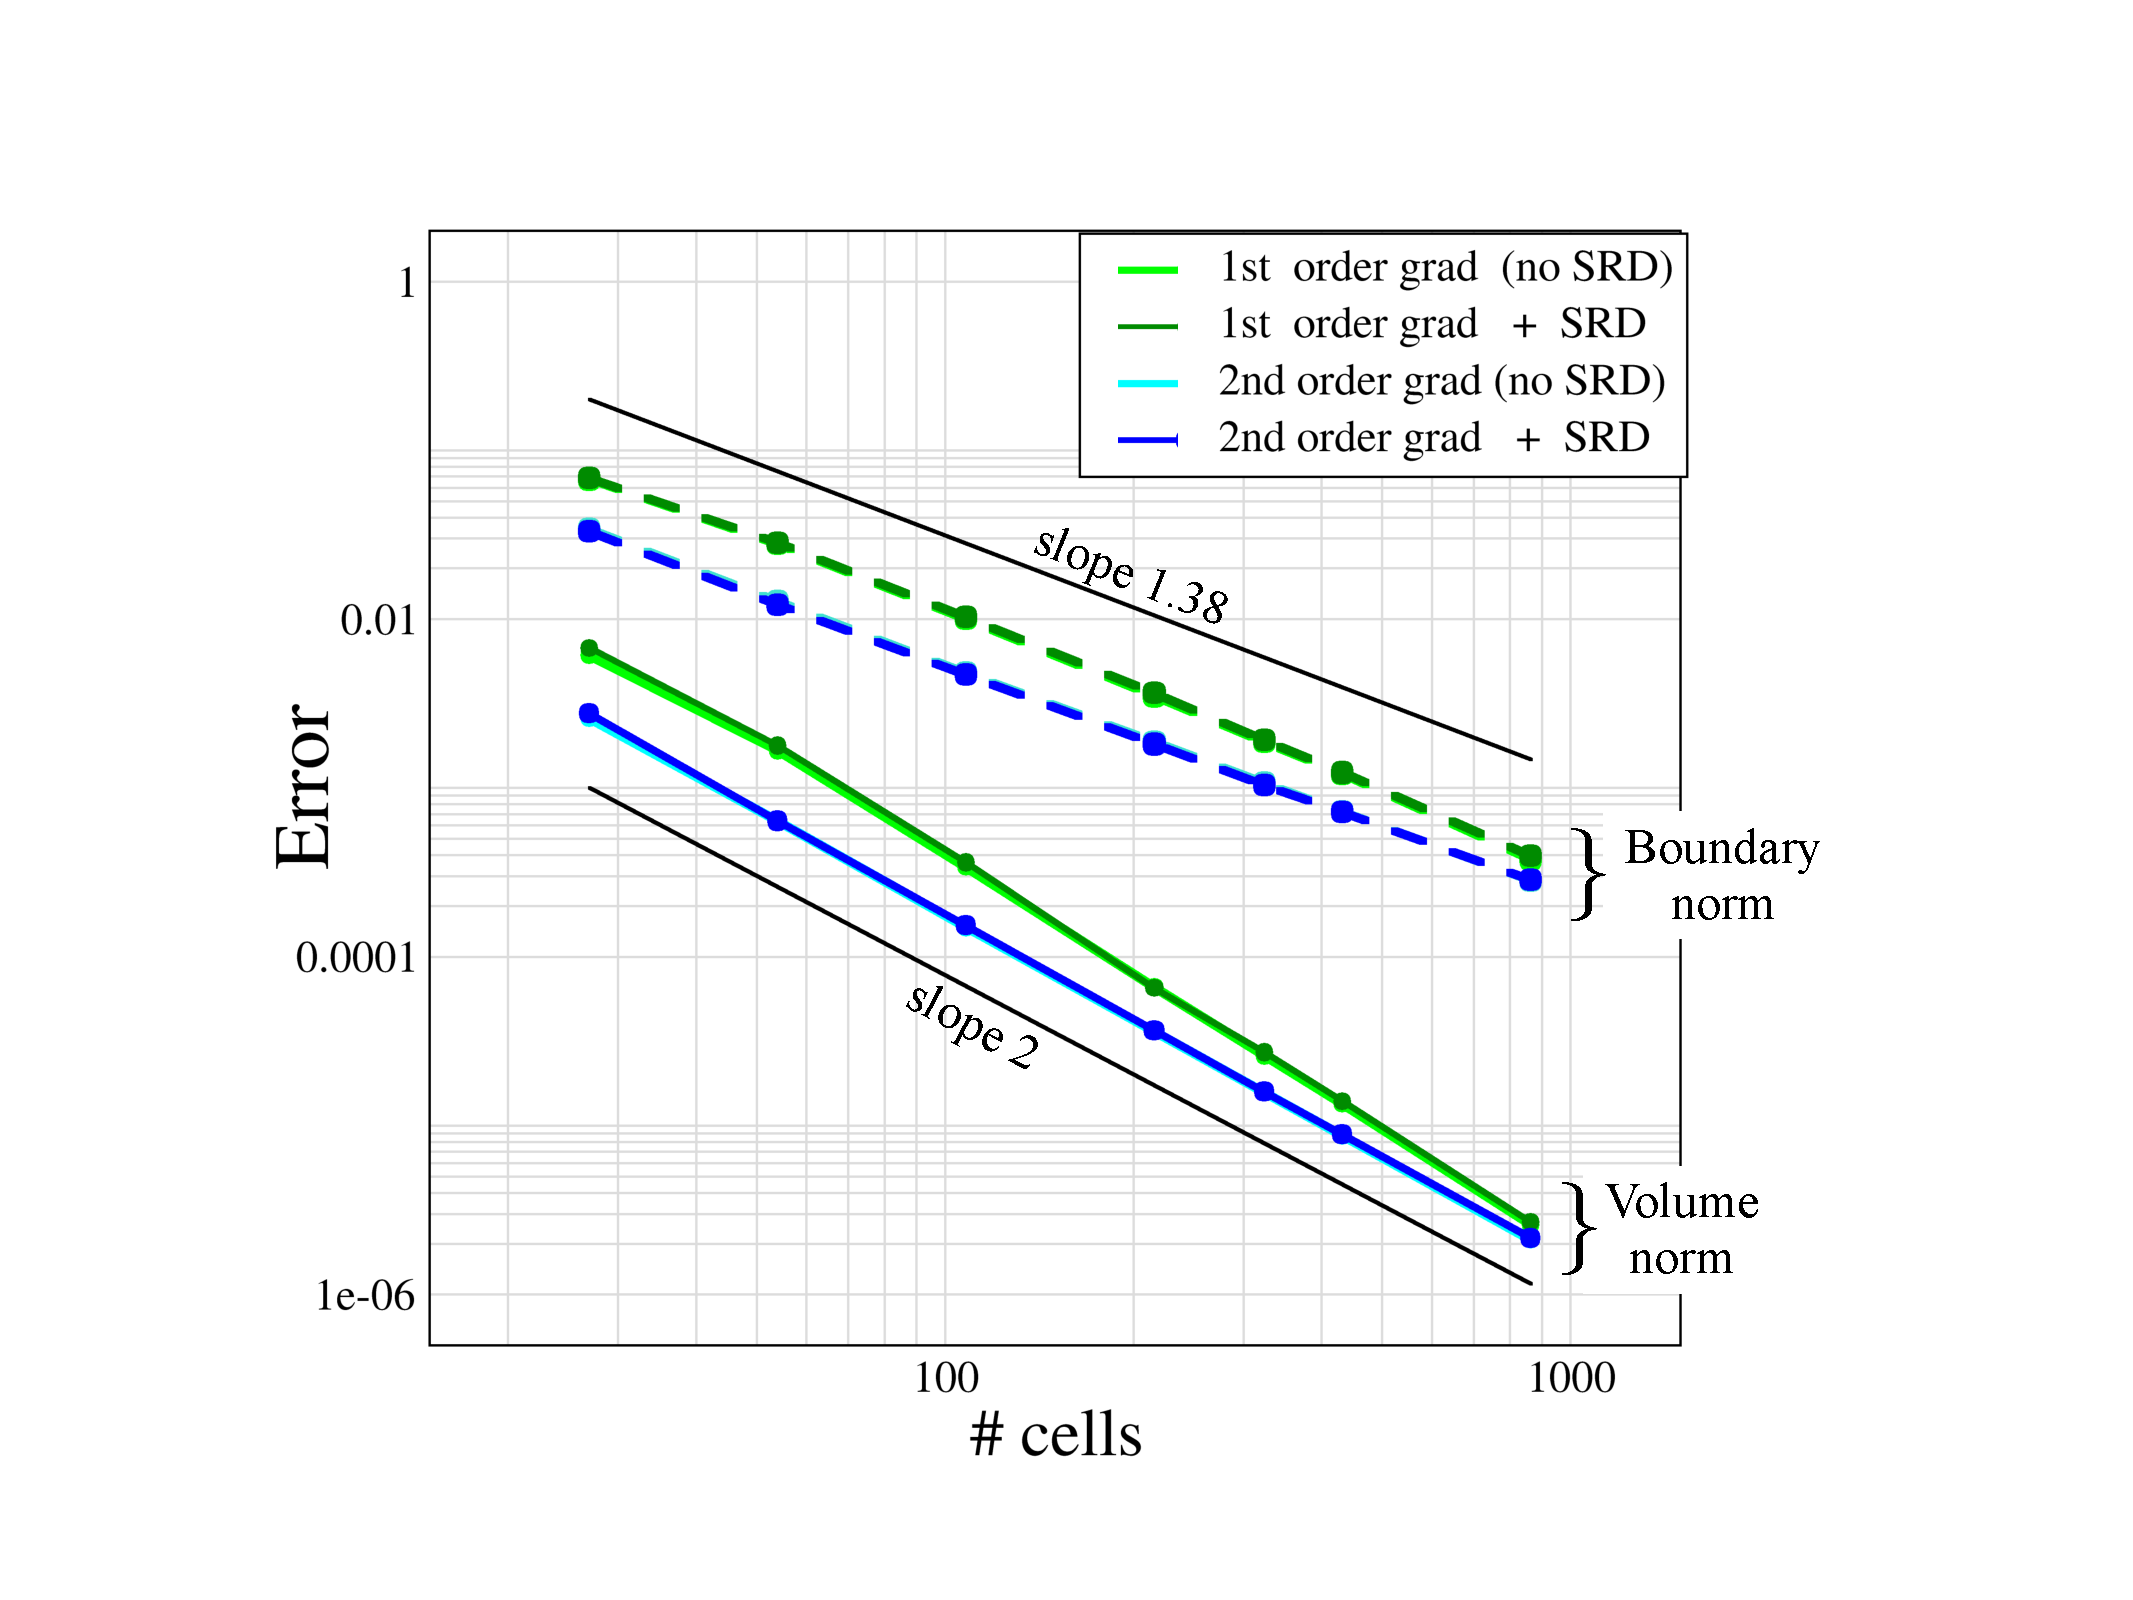
\includegraphics[height=3.0in]{figs/ssvconv.pdf}
		\caption{\sf Convergence in the L1 norm of the error in the entire 
			domain  (solid line), and along the boundary (dashed line).
			The reference line has slope 2 next to the domain error. The convergence
			rate at the boundary is between 1.38 and 1.5
			along the boundary.
			\label{fig:ssv}}
	\end{center}
\end{figure}


\clearpage

\subsection{Shock Reflection from  Cylinder}
Next we demonstrate the method for the Euler equations using a Mach 2
shock diffracting around a circular cylinder. A cylinder with radius $0.15$ is centered at
(0.5,0.5), and the shock is initially located at $x = 0.2$.
For this example we compare results using the MUSCL scheme and
the Method of Lines as the base schemes, both using local Lax Friedrichs for the Riemann
solver. The BJ limiter is used to limit
both the base scheme irregular cells  and tile reconstruction gradients. 

Figure \ref{fig:cyl1} (left) shows the solution density from MUSCL, and
right from MOL, at time $t=0.25$. 
Both grids use 302 cells in each
directions, and the domain is  $[0.0,0.0,]$ by  $[1.00001, 1.0]$, again to
prevent mesh degeneracies.
There are 416 cut cells
around the cylinder. 160 of the cut cells had volume fractions less than
0.5 and had SRD applied.  The smallest volume fraction was 1.17E-4.   
For comparison, this is also the time shown in \cite{mjb-hel-rjl:hbox2}. 

\begin{figure}[h]
\begin{center}
\vspace*{-.1in}
\hspace*{-.4in}
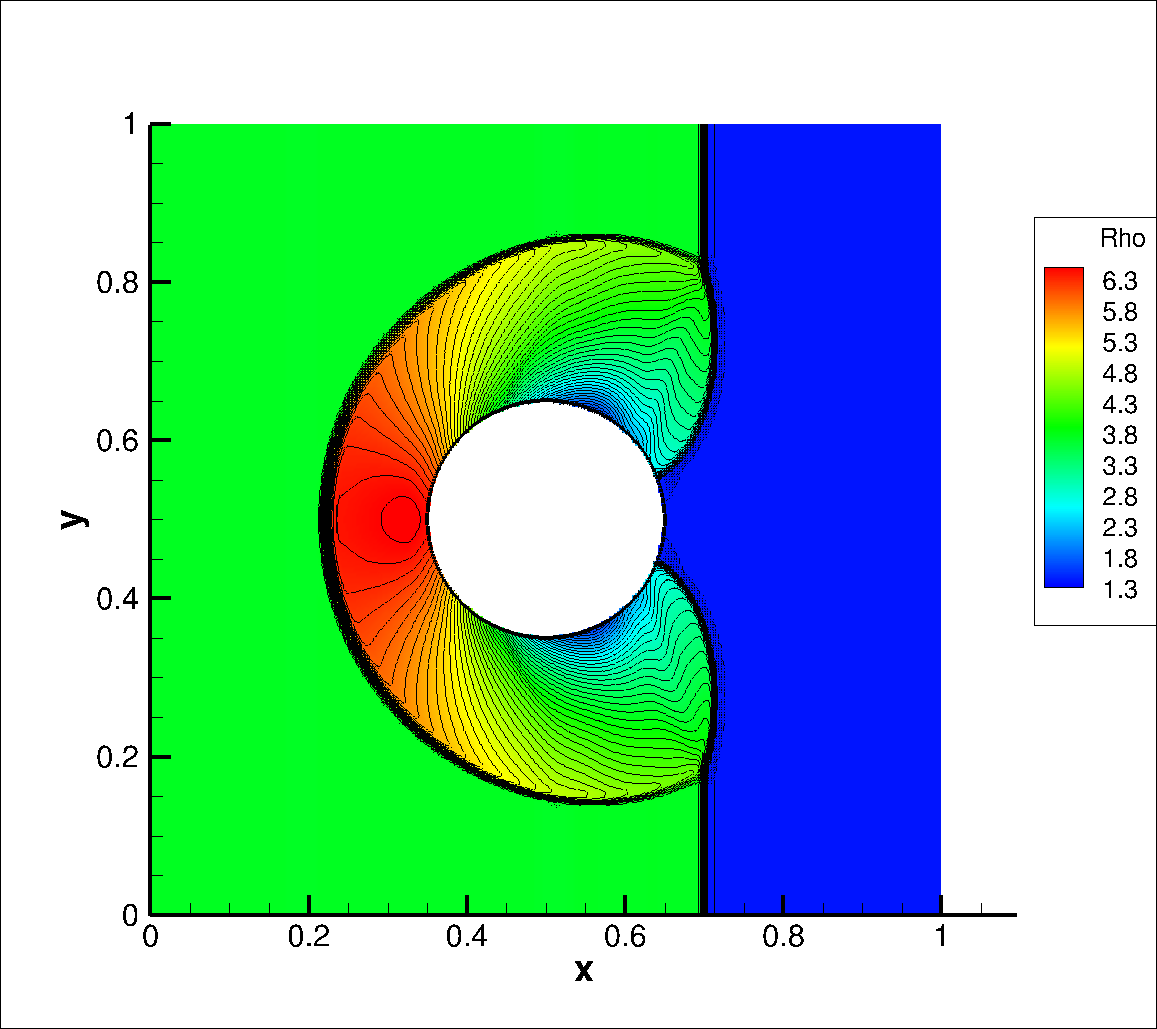
\includegraphics[width=0.48\linewidth,trim=10 10 200 10,clip]{figs/muscl_302cells.png}
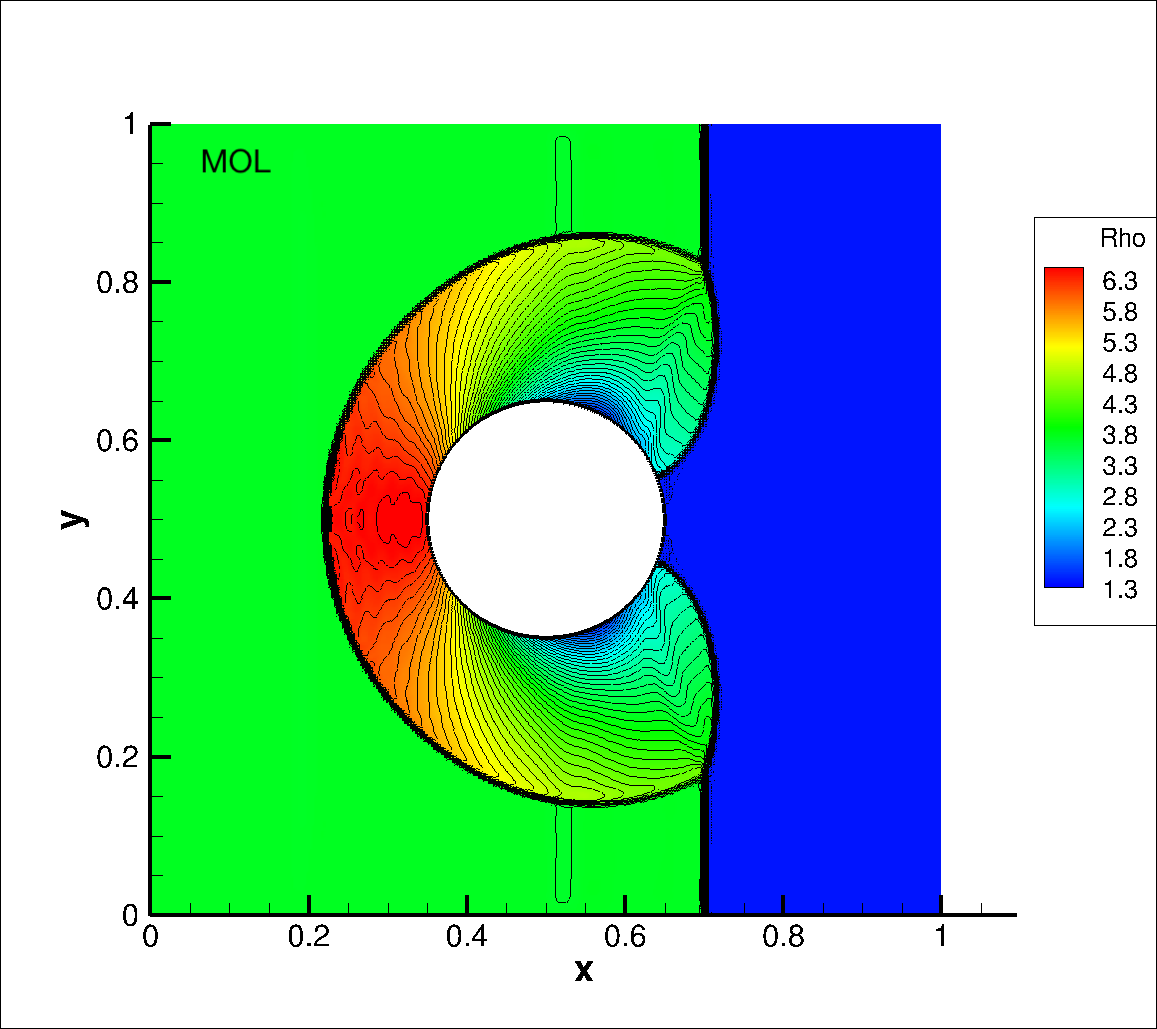
\includegraphics[width=0.48\linewidth,trim=10 10 200 10,clip]{figs/MOL_302cells.png}
\caption{\sf Density profile of Mach 2 shock reflection around a cylinder,
at time t=0.25.  Left computation used MUSCL, right used MOL. 
There are 52 contours between 1.3 and 6.5.
The front of the cylinder is better behaved with MUSCL, but the solution
at the cut cells is better  with the method of lines.
\label{fig:cyl1}}
\end{center}
\vspace*{-.1in}
\end{figure}

Figure \ref{fig:cylbndry}
shows the density profile from both schemes
taken along the cylinder.
For this plot, the cut cell variable is
reconstructed to the midpoint of the cylinder line segment in each  cell.  
The zoom shows the difference more
clearly.

\begin{figure}
\begin{center}
%\includegraphics[width=0.48\linewidth,trim=20 20 20 30,clip]{figs/densityCompare_302_normalvs3by3.png}
\hspace*{-.5in}
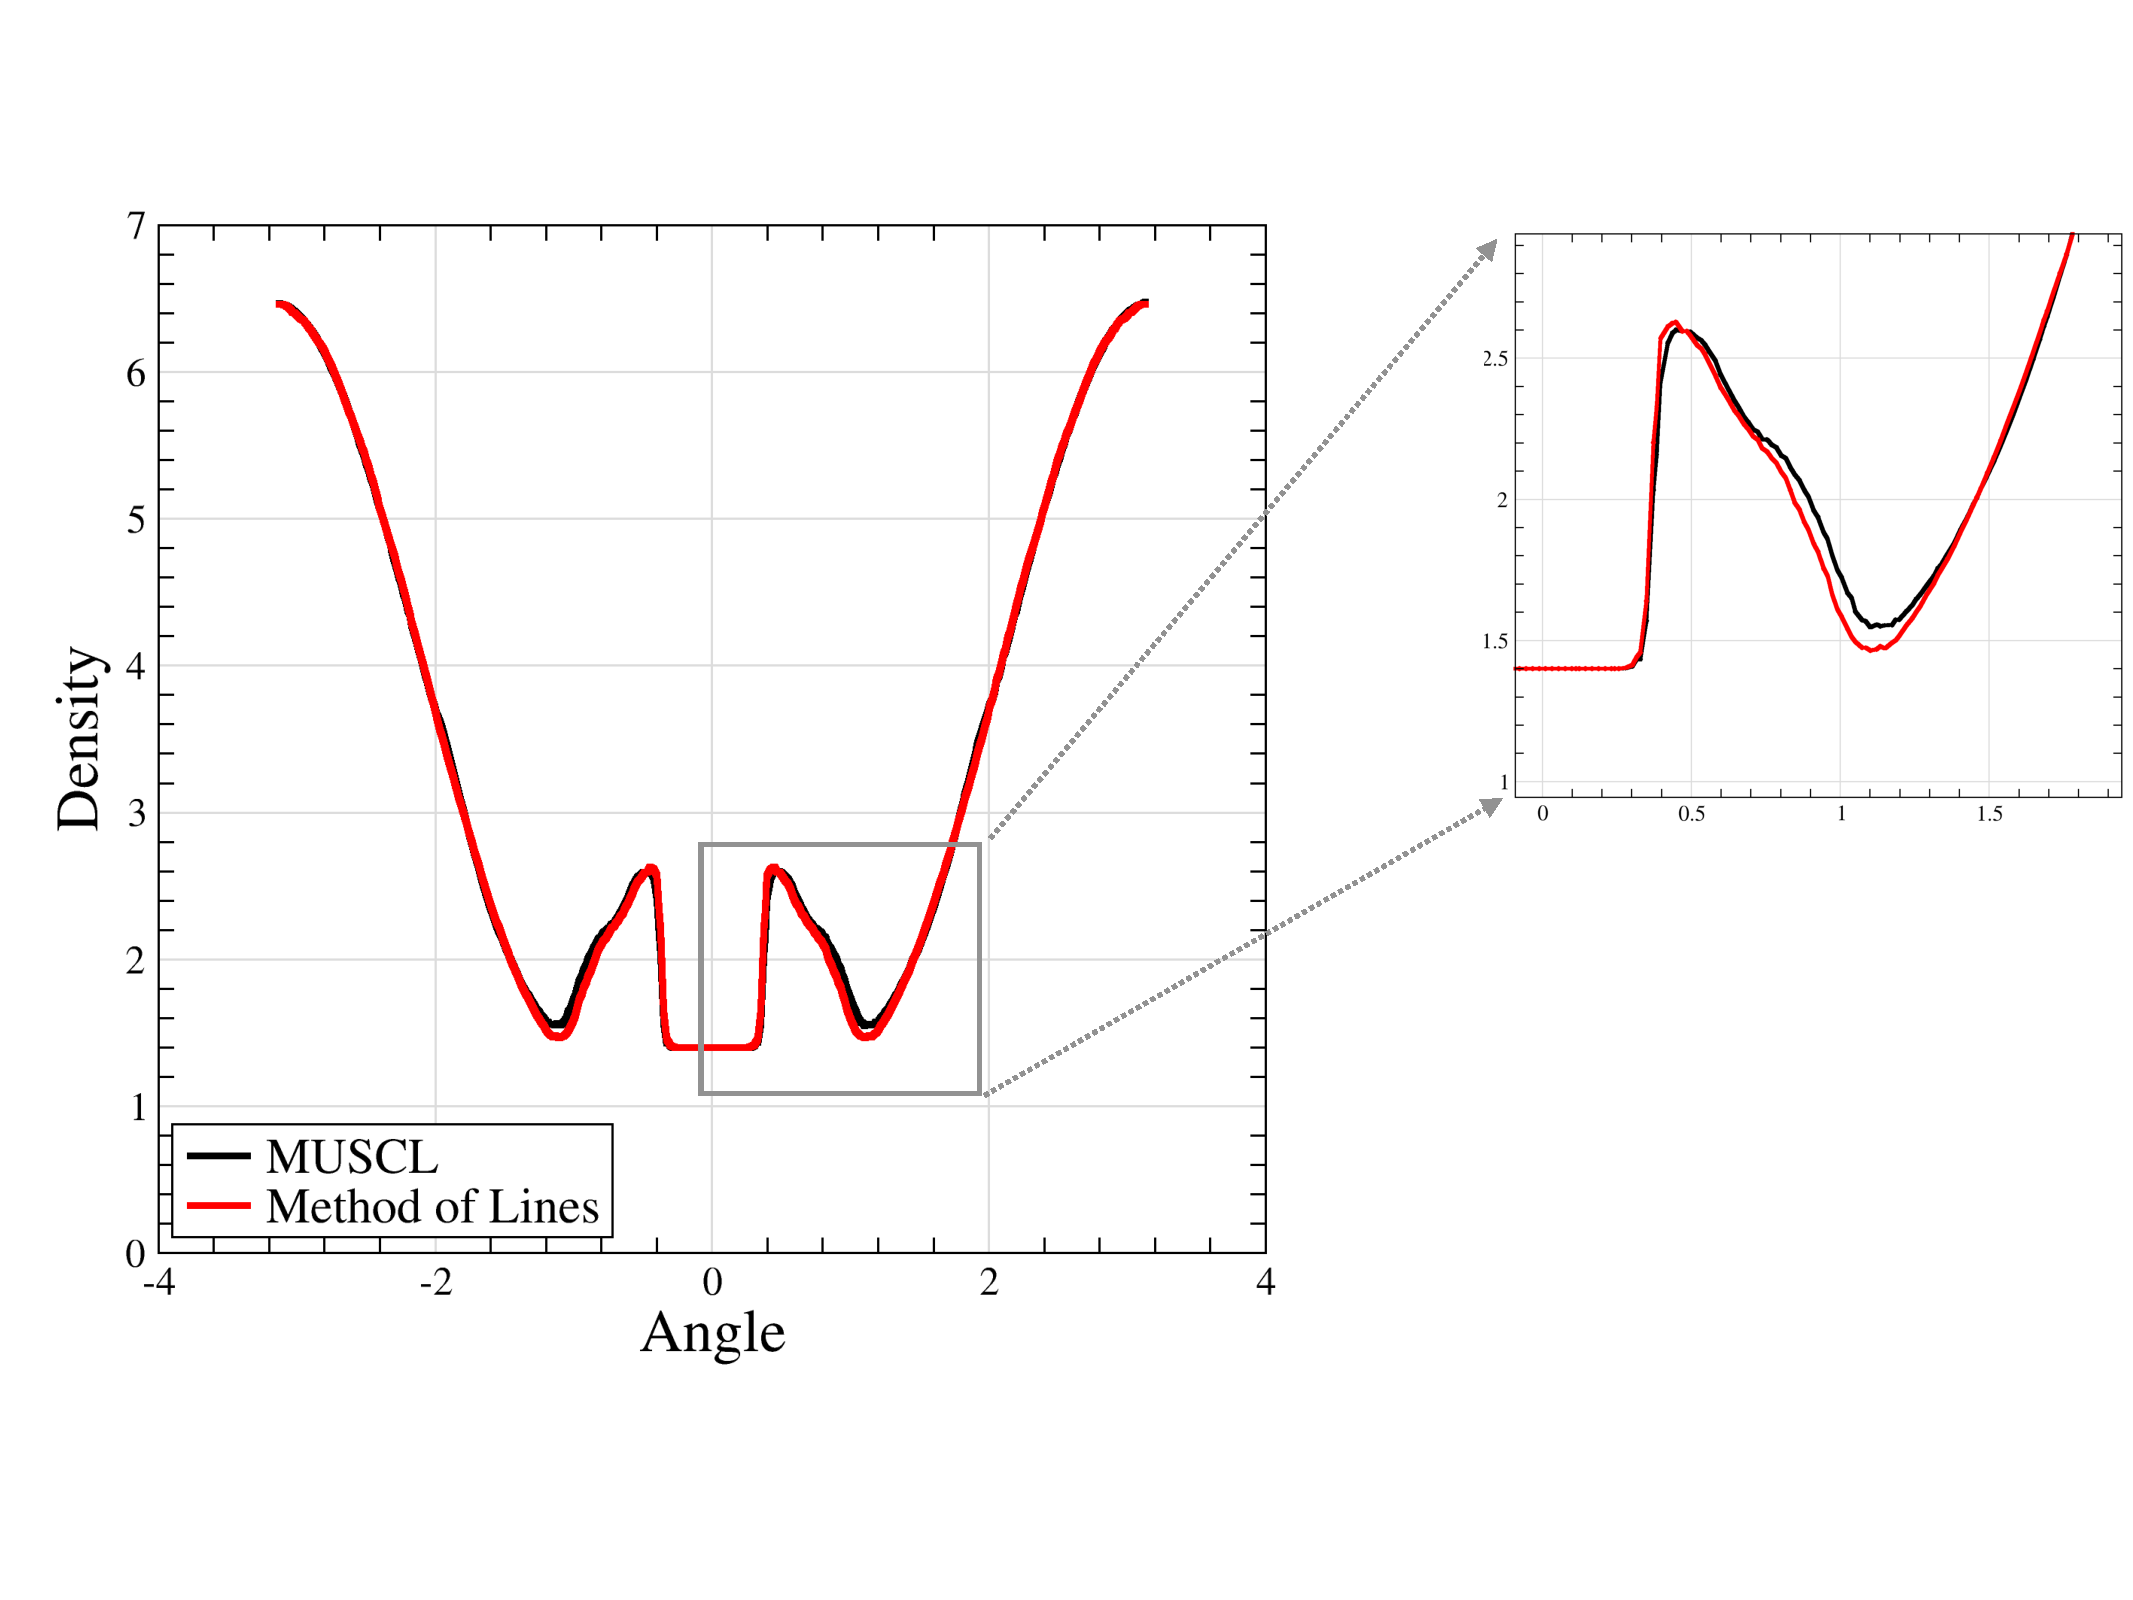
\includegraphics[height=2.7in]{figs/MM_densityBndry.pdf}
\hspace*{.3in}
%\includegraphics[width=0.48\linewidth,trim=20 20 20 30,clip]{figs/pressureCompare_302_normalvs3by3.png}
%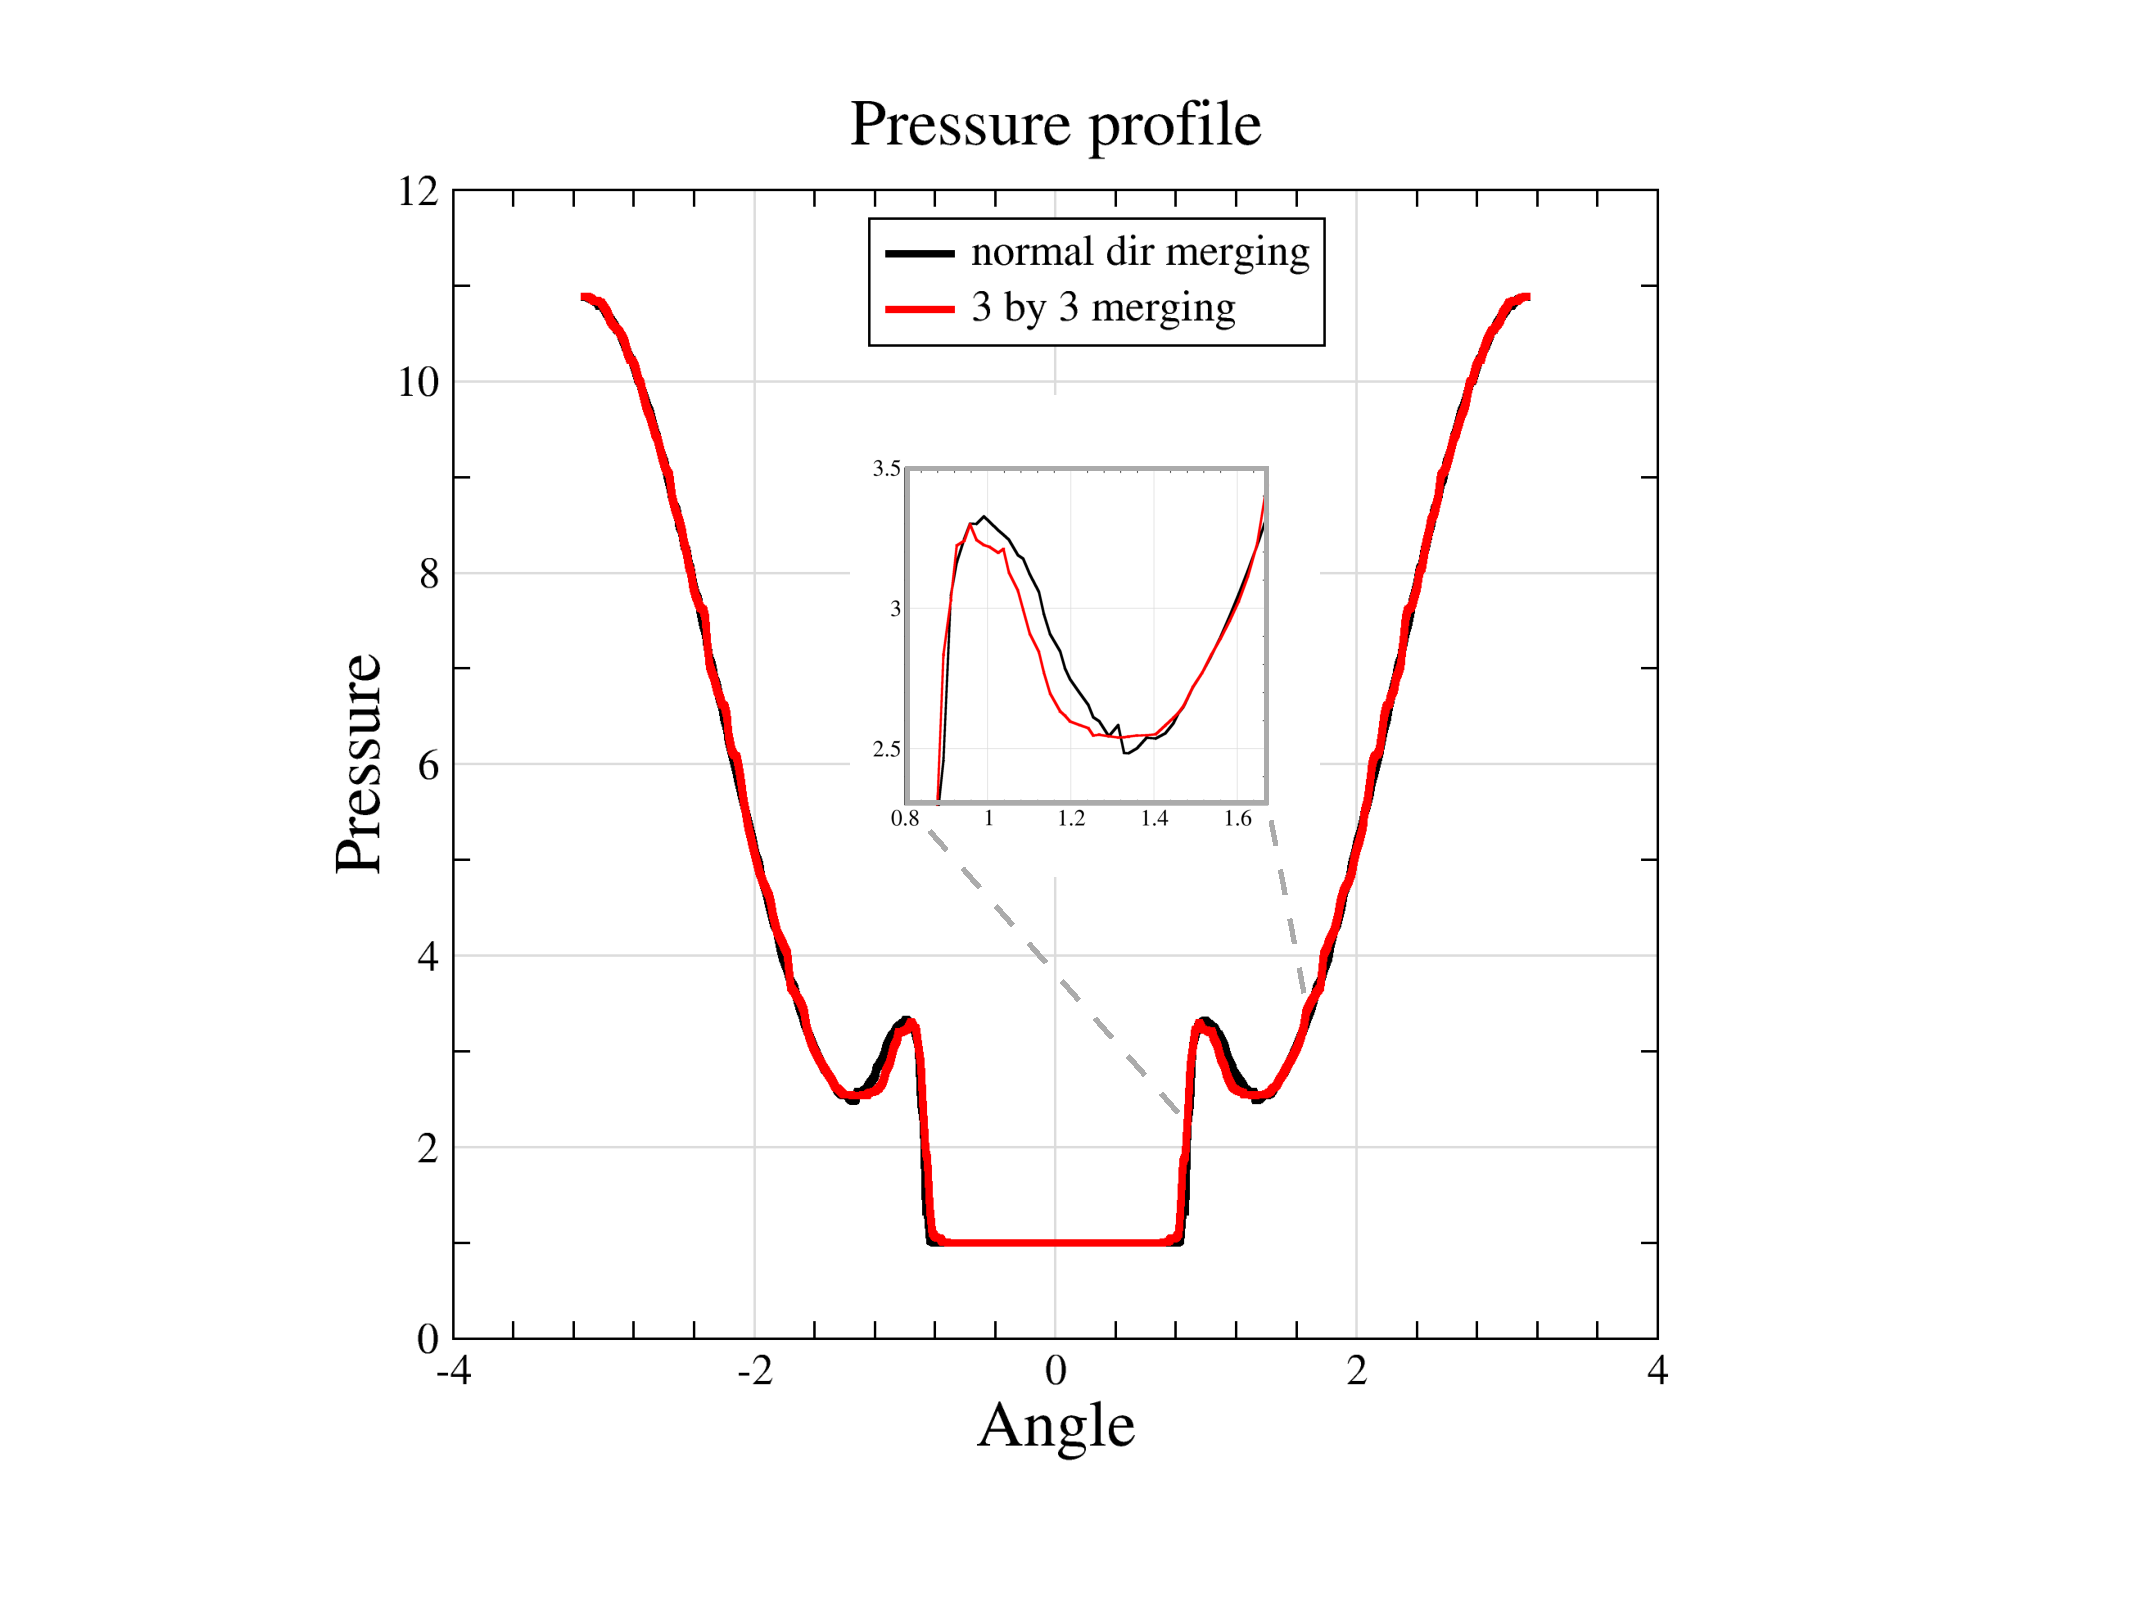
\includegraphics[height=2.7in,trim=120 70 230 50,clip]{figs/pressureWithZoom.pdf}
\caption{\sf The density profile  around the cylinder for the MUSCL and MOL schemes anat time
t=0.25.  The MOL scheme has smoother results.}
\label{fig:cylbndry}
\end{center}
% fig in amrclaw-amrcart/example/cylinder_Mach2 directory on juniper
% using sortedcyl.dat (coied from bndry01.dat) in the various _output dirs
\end{figure}

\clearpage

\subsection{Double Mach Reflection problem}
In this section, we reflect a Mach 10 shock obliquely over a wedge, where the shock and wall form a $60^{\circ}$ angle.  
This problem is solved on $[0,3]\times[0,2]$, with an angled wall embedded in the domain (Figure \ref{fig:dmnca}).  
We use the finite volume TVD-RK2 scheme with second order slopes on the base grid and neighborhoods, limited using Barth Jeserpsen.
%The goal of this test is to demonstrate that qualitatively comparable solutions are obtained, regardless of the orientation of the embedded boundary with respect to the underlying Cartesian grid.  
The solution to this problem is a complex, self-similar reflection pattern composed of incident and reflected shocks, Mach stem, and a contact discontinuity \cite{WOODWARD1984115}.  
The contact discontinuity is an unstable feature of the solution that can be difficult to resolve correctly, especially in the neighborhood of the reflecting boundary, e.g., carbuncle phenomenon \cite{KEMM2018596}.

The solution at the final time $T = 0.2$ is plotted in Figure \ref{fig:dm}, where the grid resolution is $\Delta x = \Delta y = 1/120$.

%We solve this shock reflection problem on a domain with a coordinate-aligned reflecting wall and on another domain with a non-coordinate-aligned reflecting wall.
%The former is the rectangular domain $[0,4] \times [0,1]$, where shock intersects the horizontal wall at $(0.5,0)$ (Figure \ref{fig:dmca}).

\begin{figure}
	\centering
	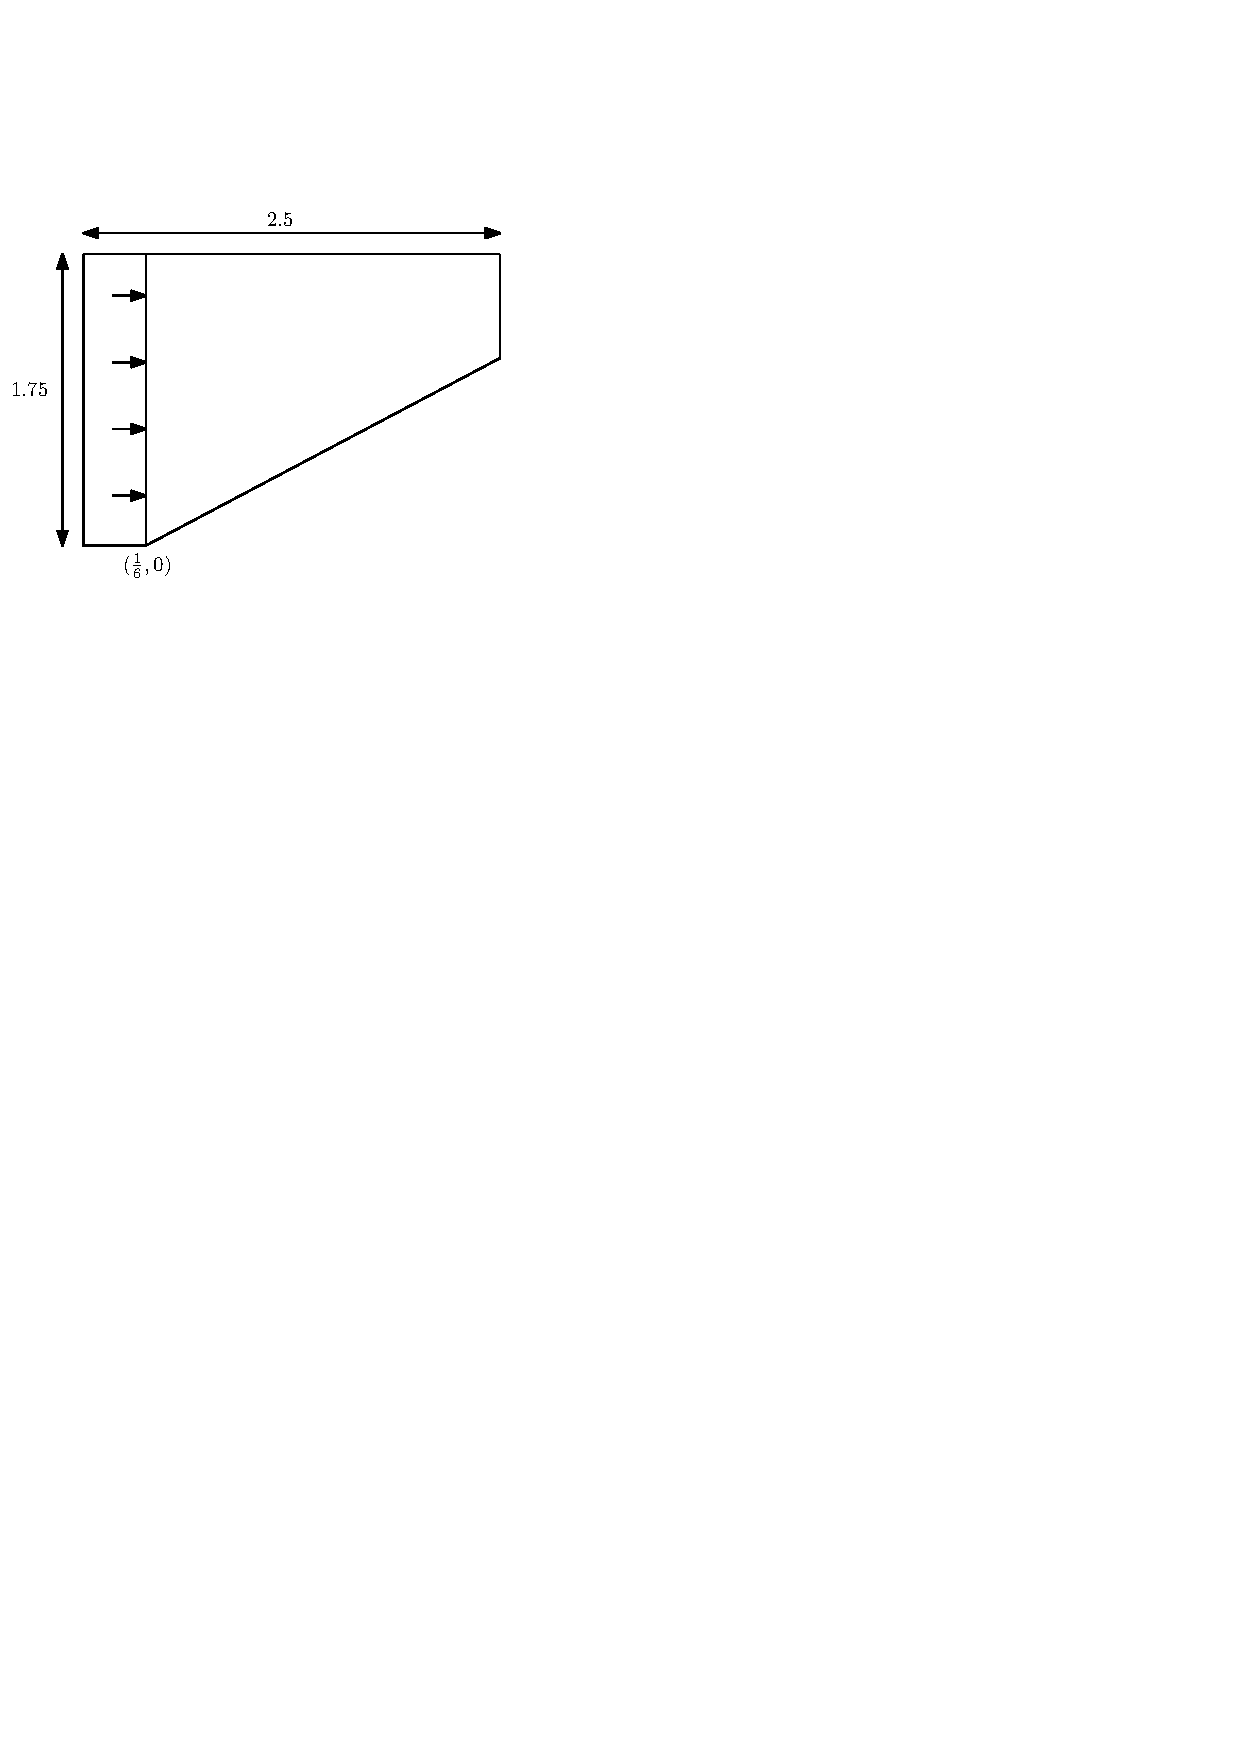
\includegraphics[width = 0.5\linewidth]{figs/dmnca}
	\caption{Non-coordinate aligned reflecting boundary.}\label{fig:dmnca}
\end{figure} 

%We plot the solution at the final time $T = 0.2$ in Figure \ref{fig:dm}.


